\chapter{CRYPTOGRAPHY TOOLS} % (fold)
\label{cha:Cryptography tools}
	% We discuss the networking and cryptographic tools used in our work.
	% referred from \cite{menezes2010handbook,stinson2005cryptography}.
	% For example, we describe the Hash function, its properties and how it helps us achieve data integrity.

	The word cryptography means ``secret writing''.
	It is the art and science of hiding the information from malicious parties.
	Cryptanalysis is the science cracking of cryptography schemes.
	Formally, the fundamental components of cryptography is a cryptosystem \cite{bishop2004introduction}.
	\begin{definition}
		A cryptosystem is a system consisting of $5$-tuple ($ \mathcal{E,D,M,K,C}$), 
		where $\mathcal{E}:\mathcal{M} \times \mathcal{K} \rightarrow \mathcal{C}$ is the set of \textit{enciphering functions}, and $\mathcal{D}:\mathcal{C} \times \mathcal{K} \rightarrow \mathcal{M}$ is the set of \textit{deciphering functions}.
		$\mathcal{M}$ is the set of \textit{plaintexts},
		$\mathcal{K}$ is the set of \textit{keys},
		$\mathcal{C}$ is the set of \textit{ciphertexts},
	\end{definition}

\section{Symmetric Key Encryption}
	% Classical cryptosystem (also called symmetric cryptosystem or single-key cryptosystem) are cryptosystem that use the same key for encipherment and decipherement.
	% In these system, for all $E_{k} \in \mathcal{C}$ and $k \in \mathcal{K}$, there is a $D_{k} \in \mathcal{D}$ such that $D_{k} = E_{k}^{-1}$.
	% \begin{definition}
	An encryption scheme made with the sets of encryption set $\{E_{e}: e \in \mathcal{K}\}$ and decryption transformations $\{D_{d}: d \in \mathcal{K}\}$, where $\mathcal{K}$ is the key space.
	The encryption scheme is said to be \textit{symmetric-key} if for each associated encryption and decryption key pair ($e,d$), it is computationally ``easy'' to determine $d$ given $e$, and to determine $e$ from $d$ \cite{menezes2010handbook}.
	In many major symmetric-key schemes satisfy $e = d$.
	% \end{definition}
	The communication protocol between two parties Alice and Bob, using symmetric key encryption scheme is shown in Figure \ref{fig:symmetric-key}. 
	The major road block with symmetric key system is to find an optimal solution to agree upon for securely doing the exchange keys between two entities, which is known as \textit{key-distribution problem} \cite{menezes2010handbook}. 

	\begin{figure}[h!]
	 	\centering
	 	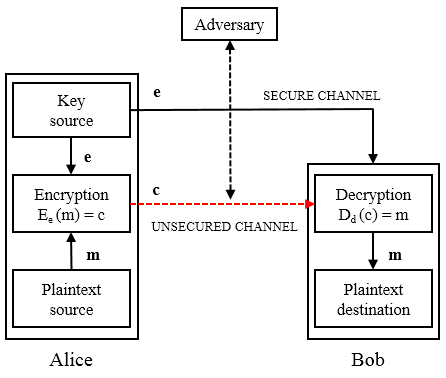
\includegraphics{images/symmetric-key.png}
	 	\caption{Two party communication using symmetric key encryption.}
	 	\label{fig:symmetric-key}
	 \end{figure} 

\section{Asymmetric/Public Key Encryption}
	Consider an encryption scheme where $\{E_{e}: e \in \mathcal{K}\}$ is a set of encryption transformations, and $\{D_{d}: d \in \mathcal{K}\}$ be the set of corresponding decryption transformations, where $\mathcal{K}$ is the key space.
	Any pair of related encryption-decryption transformations $(E_{e},D_{d})$ and assuming that each pair has the property that knowing $E_{e}$ it is computationally infeasible, given a random cipher text $c \in \mathcal{C}$, to find the message $m \in \mathcal{M}$ such that $E_{e}(m) = c$.
	It implies that given the encryption key $e$, it is impossible for an adversary to determine the related decryption key $d$.
	This is contrary to the symmetric key schemes in which $e$ and $d$ are the same\cite{menezes2010handbook}.
	The communication protocol between two parties Alice and Bob, using asymmetric key encryption scheme is shown in Figure \ref{fig:public-key}. 
	% Bob selects the key pair $(e, d)$. 
	% Bob sends the encryption key $e$ (called the \textit{public key}) to Alice over any channel but keeps the decryption key $d$ (called the \textit{private key}) secure and secret.
	% Alice may subsequently send a message $m$ to Bob and applying the encryption transformation determined by Bob's public key to get $c = E_{e}(m)$.
	\begin{figure}[h]
		\centering
		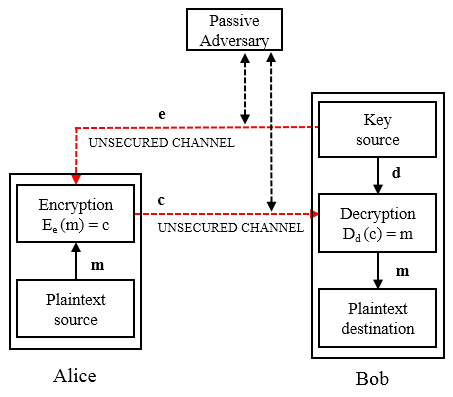
\includegraphics{images/public-key.png}
		\caption{Two party communication using asymmetric key encryption.}
		\label{fig:public-key}
	\end{figure}
	% Bob decrypts the ciphertext $c$ by applying the inverse transformation $D_{d}$ uniquely determined by $d$.
	% Here the encryption key is transmitted to Alice over an unsecured channel.
	% Since, the encryption key $e$ need not be kept secret, it may be made public.

\section{Hash Function}
	A hash function takes a message as its input and outputs a fixed length message called hash code.
	The hash code represents a compact image of the message like a digital fingerprint.
	Hash functions are essential mathematical tools to achieve data integrity.
	A hash function should have the security properties like Compression, Ease of computation, Preimage resistance, Collision resistance.
	Compression means a hash function maps an input of arbitrary finite bit length, to an output of fixed bit length $n$.
	Ease of computation means given the hash function and input, it is easy to compute the output.
	Preimage resistance means given the outputs, it is impossible to discover any input whose hashed output maps to the given output.
	Collision resistance means it is hard to construct two unique inputs which hashes to the same value.
	SHA-256, is a 256-bit hash and assures $128$ bits of security against collision attacks\cite{SHA256}.
	For most of the applications $128$ bits security is adequate.

\section{Message Authentication Codes}
	A Message Authentication Code (MAC) is a group of hash functions parameterized by a secret key $k$, also known as keyed hash function ($h_{k}$).
	It should have the security properties similar properties like Ease of computation, Compression, Computation-resistance describe for hash functions. 
	If all these properties are not satisfied then a MAC algorithm can be attacked with MAC forgery.

\section{Digital Signatures}
	\label{sec:digital-signature}
	A digital signature is a cryptographic scheme providing the security services of the authenticity, integrity and non-repudiation of a digital message. 
	A valid digital signature provides a proof to a recipient that the message was created by an authentic sender, such that the sender cannot deny having created and sent the message.
	It also guarantees that the message was not altered during the transmission.
	A Digital Signature scheme consists of the following:
	\begin{enumerate}
		\item a plain text message space $\mathcal{M}$ (set of strings over alphabets)
		\item a signature space $\mathcal{S}$ (set of possible signatures)
		\item a signing key space $\mathcal{K}$ (set of possible keys for signature generation) and a verification space $\mathcal{K^{'}}$ (a set of possible verification keys)
		\item an efficient key generation algorithm \textsf{Gen} : $N \rightarrow$ $\mathcal{K} \times \mathcal{K^{'}} $ 
		\item an efficient signing algorithm \textsf{Sign} : $ \mathcal{M} \times \mathcal{K} \rightarrow \mathcal{S}$
		\item an efficient verification algorithm \textsf{Verify} : $\mathcal{S} \times \mathcal{M} \rightarrow$ \{true, false\} 
	\end{enumerate}
	For any secret key $s_{k} \in \mathcal{K}$ and any $m \in \mathcal{M}$,	the message $m$ is signed using key $s_{k}$ as follows:
		\begin{equation}
			s = \textsf{Sign}_{s_{k}}(m)
			\label{eq:signature}
		\end{equation}
	For any $s_{k}$ let $p_{k}$ denote public key and for all $m \in \mathcal{M}$ and $s \in \mathcal{S}$, $s$ as follows:
	\begin{equation}
		\textsf{Verify}_{p_{k}}(m,s) = 
		\begin{cases}
		 \textbf{true}\ \mbox{with probability of 1} & \mbox{if}\ s = \textsf{Sign}_{s_{k}}(m)\\
		 \textbf{false}\ \mbox{with overwhelming probability} & \mbox{if}\ s \neq \textsf{Sign}_{s_{k}}(m)
		\end{cases}
		\label{eq:verification}
	\end{equation}
	where the probability space is determine by the $\mathcal {M, S, K, K^{'}}$ and perhaps the signing and verification algorithms.
	The ``overwhelming probability'' for the signature scheme determines the probability that the scheme allows for a forgery.
	In Figure \ref{fig:digita-signature}, we show the steps for signing and verifying the hashed message \cite{DigitalSignature}. 
	\begin{figure}[h]
		\centering
		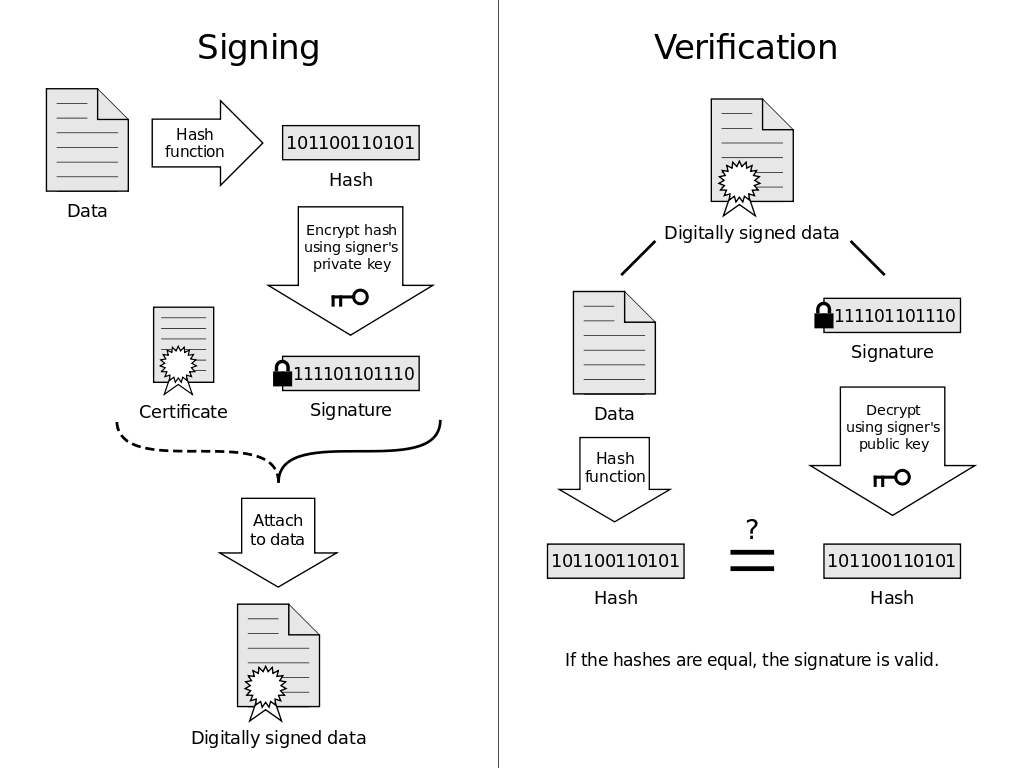
\includegraphics[scale = 0.4]{images/Digital_Signature_diagram.png}
		\caption{ Signing and verification of digital signatures}
		\label{fig:digita-signature}
	\end{figure}
	The message is hashed before its being signed to reduce the message size. 
	If the message is not hashed before signing then the signature can be longer than the message which is problematic for the longer messages.

	In the Digital Signature scheme only the owner of the secret key can generate a valid signature.
	The digital signature is easily verified by other parties as long as they know the public key.
	The digital signature is not only tied to the signer but also to the message that is being signed.
	Digital signatures do not encrypt the message. However, if necessary, a signed message can be encrypted after it is signed.

	% \textbf{Talk about non-repudiation, authenticity, integrity.}
	% \textbf{Talk about similarities and differences between physical world signature non-repudiation, authenticity, integrity.}
	% In physical world, your signatures are the same for all the messages. 
	% But this can not be possibly true for digital signatures as the attacker can obtain one signature and then use the same signature to pretend some one else.

\section{Summary}
	Three different integrity-protection mechanisms HASH, MAC, Signature can be summarized in a matrix like Table \ref{table:summary} \cite{2002-Stajano-ubiquitous}.
	These primitives differ from the partys' capabilities of generating and verifying the code which depends on the application.
	\begin{table}[!htb]	
		\caption{A comparison security primitives}
		\begin{center}
			\begin{tabular}{ |l || l| l| }
		    \hline
		     & Who can generate it & Who can verify it \\
		    \hline
		    \hline
		    Hash & Everyone & Everyone \\	
		    \hline
		    MAC & Holders of secret & Holders of secret \\
		    \hline
		    Signature & Holder of secret & Everyone \\
		    \hline
			\end{tabular}
		\end{center}
	  \label{table:summary}
	\end{table}

% \section {Tree generation algorithms}

% \section{XOR function}

% \section{Elliptic curve}